\documentclass[a4paper]{article}
\usepackage{amsmath}
\usepackage{amssymb}
\usepackage{xcolor}
\usepackage{amsthm}
\usepackage{dsfont}
\usepackage{graphicx}
\usepackage{hyperref}
\usepackage{datetime}
\usepackage{outlines}
\usepackage{float}
\usepackage{booktabs}
\usepackage{enumitem}


\definecolor{fgcolor}{rgb}{0.345, 0.345, 0.345}
\newcommand{\hlnum}[1]{\textcolor[rgb]{0.686,0.059,0.569}{#1}}%
\newcommand{\hlstr}[1]{\textcolor[rgb]{0.192,0.494,0.8}{#1}}%
\newcommand{\hlcom}[1]{\textcolor[rgb]{0.678,0.584,0.686}{\textit{#1}}}%
\newcommand{\hlopt}[1]{\textcolor[rgb]{0,0,0}{#1}}%
\newcommand{\hlstd}[1]{\textcolor[rgb]{0.345,0.345,0.345}{#1}}%
\newcommand{\hlkwa}[1]{\textcolor[rgb]{0.161,0.373,0.58}{\textbf{#1}}}%
\newcommand{\hlkwb}[1]{\textcolor[rgb]{0.69,0.353,0.396}{#1}}%
\newcommand{\hlkwc}[1]{\textcolor[rgb]{0.333,0.667,0.333}{#1}}%
\newcommand{\hlkwd}[1]{\textcolor[rgb]{0.737,0.353,0.396}{\textbf{#1}}}%
\let\hlipl\hlkwb

\usepackage{framed}
\makeatletter
\newenvironment{kframe}{%
 \def\at@end@of@kframe{}%
 \ifinner\ifhmode%
  \def\at@end@of@kframe{\end{minipage}}%
  \begin{minipage}{\columnwidth}%
 \fi\fi%
 \def\FrameCommand##1{\hskip\@totalleftmargin \hskip-\fboxsep
 \colorbox{shadecolor}{##1}\hskip-\fboxsep
     % There is no \\@totalrightmargin, so:
     \hskip-\linewidth \hskip-\@totalleftmargin \hskip\columnwidth}%
 \MakeFramed {\advance\hsize-\width
   \@totalleftmargin\z@ \linewidth\hsize
   \@setminipage}}%
 {\par\unskip\endMakeFramed%
 \at@end@of@kframe}
\makeatother

\definecolor{shadecolor}{rgb}{.97, .97, .97}
\definecolor{messagecolor}{rgb}{0, 0, 0}
\definecolor{warningcolor}{rgb}{1, 0, 1}
\definecolor{errorcolor}{rgb}{1, 0, 0}
\newenvironment{knitrout}{}{} % an empty environment to be redefined in TeX


% code highlighting
\usepackage{minted}
\usepackage{xpatch}
\newminted[cminted]{python}{fontsize=\small}
\xpretocmd{\cminted}{\RecustomVerbatimEnvironment{Verbatim}{BVerbatim}{}}{}{}

% link coloring
%\hypersetup{
%    colorlinks,
%    linkcolor={red!80!black},
%    citecolor={green!60!black},
%    urlcolor={blue!80!black}
%}

% concatenation symbol (c.f. ++ in Haskell)
\newcommand\mdoubleplus{\mathbin{+\mkern-10mu+}}

% end of proof symbol
\newcommand{\newmarkedtheorem}[1]{%
  \newenvironment{#1}
    {\pushQED{\qed}\csname inner@#1\endcsname}
    {\popQED\csname endinner@#1\endcsname}%
  \newtheorem{inner@#1}%
}

\theoremstyle{definition}
%\newtheorem{eg}{Example}[section]
\newmarkedtheorem{eg}{Example}[section]
\newtheorem{observation}{Observation}[section]
\newtheorem{define}{Definition}[section]
\theoremstyle{plain}
\newtheorem{proposition}{Proposition}
\newtheorem{lemma}{Lemma}
\newtheorem{corollary}{Corollary}
\newtheorem{theorem}{Theorem}[section]
\newtheorem{assump}{Assumption}[section]
\newtheorem{remark}{Remark}[section]

\newdateformat{monthyeardate}{\monthname[\THEMONTH] \THEYEAR}

\author{Jeroen van Riel}
\date{\monthyeardate\today}
\title{}

\begin{document}

\section*{Single Intersection}

We first emphasize that the vehicle dynamics we use is equivalent to the common
\textit{double integrator} model from optimal control theory. This part is
mainly for my own understanding and is not necessary for the remaining
dicussion. We then define a single intersection model with incoming lanes and
the general problem of finding optimal trajectories. Vehicles are not able to
overtake one another in this model. We briefly show how direct transcription can
be used to turn the infinite-dimensional optimization problem into a
mixed-convex program that modern off-the-shelf solvers can turn into a solution.

Next, we argue that we can forget about the vehicle dynamics when the objective
function only involves, for each vehicle, the time it crosses the intersection.
The rest of the report discusses branch-and-bound methods and heuristics for
solving the resulting scheduling problem.

{\color{blue} Comments and ideas for further work are in blue.}


\subsection*{Vehicle dynamics}

In control theory, it is common to model motion dynamics of a system in terms of
a state vector $s(t) \in \mathbb{R}^{n}$ and a control input vector
$u(t) \in \mathbb{R}^{m}$, which result in a scalar position $y(t)$ via the
equations
\begin{subequations}\label{eq:control_equations}
\begin{align}
  \dot{s}(t) &= A s(t) + B u(t) , \\
  y(t) &= C s(t) .
\end{align}
\end{subequations}
%
Furthermore, the state and control trajectories are often restricted by imposing
linear constraints of the form
\begin{subequations}\label{eq:control_constraints}
\begin{align}
  G s(t) \leq b , \\
  F u(t) \leq d .
\end{align}
\end{subequations}
%
In the discussion that follows, each vehicle is modeled as a \textit{double integrator},
with $s(t) = (p(t), v(t))$, where $p(t)$ and $v(t)$ are the scalar position
along a predefined path and corresponding velocity, respectively. The three
matrices are chosen such that
\begin{align*}
  \dot{s}(t) &= \begin{pmatrix} 0 & 1 \\ 0 & 0 \end{pmatrix} s(t) + \begin{pmatrix} 0 \\ 1 \end{pmatrix} u(t), \\
  y(t) &= \begin{pmatrix} 1 & 0 \end{pmatrix} s(t),
\end{align*}
which may simply be rewritten as
\begin{align}
  \label{eq:motion_dynamics}
  \dot{p}(t) = v(t) , \quad
  \dot{v}(t) = u(t) , \quad
  y(t) = p(t) ,
\end{align}
where we recognize that the control input $u(t)$ corresponds directly to the
acceleration of the vehicle.


\subsection*{Intersection model}

Consider an intersection with $n$ incoming lanes. We define the index set
\begin{align*}
  \mathcal{N} = \{ (l, k) : k \in \{1, \dots, n_{l}\}, \; l \in \{1, \dots n\}\} ,
\end{align*}
where $n_{l}$ denotes the number of vehicles of lane $l$. To
further help with notation, given vehicle index $i = (r,s) \in \mathcal{N}$, we
define $l(i) = r$ and $k(i) = s$.

We assume that the position $p_{i}(t)$ of some vehicle $i \in \mathcal{N}$
corresponds to the physical front of the vehicle.
%
In order to model a safe distance between vehicles on the same lane, we require
that
\begin{align*}
  p_{i}(t) - p_{j}(t) \geq P_{i} ,
\end{align*}
for all $t$ and all pairs of indices $i, j \in \mathcal{N}$ such that
$l(i) = l(j), \; k(i) + 1 = k(j)$, with $P_{i} \geq 0$. Let $\mathcal{C}$ denote
the set of such ordered pairs of indices. Note that these constraints restrict
vehicles from overtaking each other.
%
Furthermore, in order to model collision avoidance, we say that a vehicle \textit{occupies the intersection}
whenever $p_{i}(t) \in [L, H_{i}] = \mathcal{E}_{i}$. The collision avoidance constraints are
given by
\begin{align*}
  (p_{i}(t), p_{j}(t)) \notin \mathcal{E}_{i} \times \mathcal{E}_{j},
\end{align*}
for all $t$ and for all pairs of indices $i, j \in \mathcal{N}$ with
$l(i) \neq l(j)$, which we collect in the set $\mathcal{D}$. Note that the length
of a vehicle can be modeled by choosing $H_{i}$ and $P_{i}$ appropriately.
%
Let $D_{i}(s_{i,0})$ denote the set of feasible trajectories
$x_{i}(t) = (s_{i}(t), u_{i}(t))$ given some initial state
$s_{i,0} = (p_{i}(0), v_{i}(0))$ and satisfying the vehicle dynamics given by
equations~\eqref{eq:motion_dynamics}. Given some performance criterion
$J(x_{i})$, the type of coordination problem we want to study is of the form
\begin{subequations}\label{eq:full_problem}
\begin{align}
  \min_{\mathbf{x}(t)} \quad & \sum_{i \in \mathcal{N}} J(x_{i}) \\
  \text{s.t.} \quad  & x_{i} \in D_{i}(s_{i,0}) , &\text{for all } i \in \mathcal{N} , \\
                & p_{i}(t) - p_{j}(t) \geq P_{i}, &\text{for all } (i,j) \in \mathcal{C} , \label{eq:follow_constraints} \\
                & (p_{i}(t), p_{j}(t))  \notin \mathcal{E}_{i} \times \mathcal{E}_{j} , &\text{for all } \{i,j\} \in \mathcal{D} \label{eq:collision_constraints} ,
\end{align}
\end{subequations}
where $\mathbf{x}(t) = [\, x_{i}(t) : i \in \mathcal{N} \,]$.

\subsection*{Direct transcription}

Optimization problem~\eqref{eq:full_problem} can be transcribed directly into a
non-convex mixed-integer linear program by discretization on a uniform time
grid. Let $K$ denote the number of discrete time steps and let $\Delta t$ denote
the time step size.
%
Using the forward Euler integration scheme, we have
\begin{align*}
  p_{i}(t + \Delta t) = p_{i}(t) + v_{i}(t) \Delta t , \\
  v_{i}(t + \Delta t) = v_{i}(t) + u_{i}(t) \Delta t ,
\end{align*}
for each $t \in (0, \Delta t, \dots, K \Delta t)$. The disjunctive constraints are formulated
using the well-known big-M technique by the constraints
\begin{align*}
  p_{i}(t) \leq L + \delta_{i}(t) M , \\
  H - \gamma_{i}(t) M \leq p_{i}(t) , \\
  \delta_{i}(t) + \delta_{j}(t) + \gamma_{i}(t) + \gamma_{j}(t) \leq 3 ,
\end{align*}
where $\delta_{i}(t), \gamma_{i}(t) \in \{ 0, 1 \}$ for all $i \in \mathcal{N}$
and $M$ is a sufficiently large number.
%
Finally, the follow constraints can simply be added as
\begin{align*}
  p_{i}(t) - p_{j}(t) \geq P_{i} ,
\end{align*}
for each $t \in (0, \Delta t, \dots, K \Delta t)$ and each pair of consecutive
vehicles $(i, j) \in \mathcal{C}$.

For example, consider the objective functional
\begin{align*}
  J(x_{i}) = \int_{t=0}^{t_{f}} \left( {(v_{d} - v_{i}(t))}^{2} + {u_{i}(t)}^{2} \right) dt ,
\end{align*}
where $v_{d}$ is some reference velocity and $t_{f}$ denotes the final time. For
example, see the optimal trajectories in
Figure~\ref{fig:direct_transcription_example}.

\begin{table}[H]
  \centering
\begin{tabular}{ c | c c c | c c }
  $i$  & (1,1) & (1,2) & (1,3) & (2,1) & (2,2) \\
  \hline
  $p_{i}$ & 15 & 10 &  0 & 10 &  0 \\
  $v_{i}$ & 10 & 10 & 10 & 10 & 10 \\
\end{tabular}
\caption{Example initial conditions for problem~\eqref{eq:full_problem}.}
\label{tab:hult_parameters}
\end{table}

\begin{figure}[H]
  \centering
  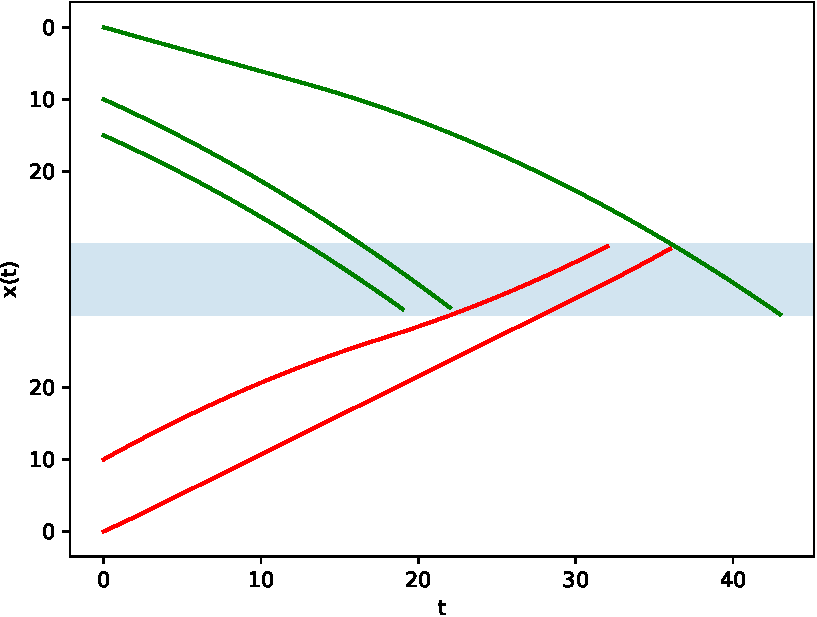
\includegraphics[width=0.8\textwidth]{figures/single/trajectories_general.pdf}
  \caption{Example of optimal trajectories obtained using the direct
    transcription method with
    $P_{i} = P = 5, \mathcal{E}_{i} = \mathcal{E} = [50, 70], v_{d} = 20, T=120, \Delta t = 0.1$
    and initial conditions as given in Table~\ref{tab:hult_parameters}. The
    y-axis is split such that each part corresponds to one of the two lanes and
    the trajectories are inverted accordingly and drawn with separate colors.
    The intersection area $\mathcal{E}$ is drawn as a shaded region. Whenever a
    vehicle has left the intersection, we stop drawing its trajectory for
    clarity.}
  \label{fig:direct_transcription_example}
\end{figure}


\subsection*{Crossing time criterion}

We start by considering a subclass of problems that allow us to almost ignore
the vehicle dynamics. As performance criterion, we consider the \textit{crossing
  time}
\begin{align}
  \label{eq:crossing_time_criterion}
  J(x_{i}) = \inf_{t} \{ t : p_{i}(t) = L \} .
\end{align}
Furthermore, we impose a maximum speed for every vehicle, so
\begin{align}
  \label{eq:max_speed_constraint}
  v_{i}(t) \leq v_\text{max} ,
\end{align}
for every $t$. We do not define any linear constraints on the control input, so
we assume \textit{instantaneous acceleration} is possible. For the purpose of
the following discussion, it is not necessary to rigorously define what we mean
by that. Define the \textit{earliest crossing time} of vehicle $i$ as
\begin{align*}
  r_{i} = &\inf_{x_{i}} J(x_{i}) \\
  &\text{s.t. } x_{i} \in D_{i}(s_{i,0})
\end{align*}
It is not hard to see that we must have $r_{i} = (L - p_{i}(0)) / v_\text{max}$.
%
Instead of optimizing in terms of trajectories $\mathbf{x}$, we consider first
finding a \textit{schedule} $y$ for the crossing times by solving
\begin{subequations}\label{eq:single_intersection_scheduling}
\begin{align}
  \min_{y} \quad & \sum_{i \in \mathcal{N}} y_{i} & \\
  \text{s.t.} \quad & r_{i} \leq y_{i} & \text{ for all } i \in \mathcal{N} , \\
  & y_{i} + \rho_{i} \leq y_{j} & \text{ for all } (i,j) \in \mathcal{C} , \label{eq:conjunctions} \\
  & y_{i} + \sigma_{i} \leq y_{j} \text{ or } y_{j} + \sigma_{j} \leq y_{i} & \text{ for all } \{i,j\} \in \mathcal{D} , \label{eq:disjunctions}
\end{align}
\end{subequations}
where $\rho_{i} = P_{i} / v_{\text{max}}$ and
$\sigma_{i} = (H_{i} - L) / v_{\text{max}}$.
%By using the well-known big-M method,~\eqref{eq:single_intersection_scheduling} can be turned into a mixed-integer program, for which solvers are readily available.
%
Note that an instance $s$ of~\eqref{eq:single_intersection_scheduling} is completely characterized by the tuple
\begin{align*}
  s = (\mathcal{N}, \rho, \sigma, r) .
\end{align*}


\begin{proposition}
  The coordination problem~\eqref{eq:full_problem} with performance criterion~\eqref{eq:crossing_time_criterion} and maximum speed
  constraints~\eqref{eq:max_speed_constraint} is equivalent with~\eqref{eq:single_intersection_scheduling}.
\end{proposition}
\begin{proof}
  We show that any feasible solution can be translated to a feasible solution to
  the other problem without changing the objective value.

  Consider a set of trajectories $\mathbf{x}(t)$. Consider some arbitrary
  vehicle $i \in \mathcal{N}$. It follows directly from the definition of $r_{i}$
  that we must have $J(x_{i}) \geq r_{i}$.
  %
  % conjunctions
  Consider a pair of consecutive vehicles $(i,j) \in \mathcal{C}$ on the same
  lane. For every $t \geq J(x_{i})$, trajectory $x_{i}$ must satisfy
  \begin{align*}
    p_{i}(t) \leq L + (t - J(x_{i})) v_{\text{max}}
  \end{align*}
  and by the constraint~\eqref{eq:follow_constraints}, trajectory $x_{j}$ must satisfy
  \begin{align*}
    p_{j}(t) \leq L + (t - J(x_{i})) v_{\text{max}} - P_{i} .
  \end{align*}
  Hence, we have $p_{j}(t) \leq L$ if and only if
  $t \leq J(x_{i}) + P_{i} / v_{\text{max}}$, which implies that
  $J(x_{j}) \geq J(x_{i}) + \rho_{i}$.
  %
  % disjunctions
  Consider a pair of vehicles $\{i, j\} \in \mathcal{D}$ on distinct lanes. By a
  similar reasoning, constraint~\eqref{eq:collision_constraints} implies that we have either
  $J(x_{i}) + \sigma_{i} \leq J(x_{j})$ or $J(x_{j}) + \sigma_{j} \leq J(x_{i})$.
  %
  %
  This shows that $y_{i} = J(x_{i})$ is a feasible schedule for~\eqref{eq:single_intersection_scheduling}.

  % schedule
  Now consider a feasible schedule $y_{i}$. For every $i \in \mathcal{N}$, we
  construct a trajectory $x_{i}$ such that $J(x_{i}) = y_{i}$ by setting
  $p_{i}(t) = p_{i}(0) + t (L - p_{i}(0)) / y_{i}$ for $0 \leq t < y_{i}$ and
  $p_{i}(t) = L + (t - y_{i}) v_{\text{max}}$ for $t \geq y_{i}$, so
  instantaneous acceleration is happening at $t=0$ and $t=y_{i}$.
  {\color{blue} This construction argument is not yet correct. Consider what happens when some lane overflows.}
\end{proof}

When we consider bounded acceleration, the trajectory generation is less
straightforward. Given the position and velocity at some start and end points,
the trajectory can be formulated as the solution of some linear
program~\cite{miculescuPollingsystemsbasedAutonomousVehicle2016}. These
results allow us to reduce the problem again to the problem of scheduling
crossing times.
\begin{proposition}
  The coordination problem~\eqref{eq:full_problem} with performance
  criterion~\eqref{eq:crossing_time_criterion}, maximum speed
  constraints~\eqref{eq:max_speed_constraint} and maximum acceleration
  constraints
  \begin{align*}
    a_{\min} \leq a_{i}(t) \leq a_{\max} ,
  \end{align*}
  for all times $t$ and vehicles $i \in \mathcal{N}$, is equivalent
  with~\eqref{eq:single_intersection_scheduling}.
\end{proposition}


\subsection*{Crossing order}

Instances and solutions of the crossing time optimization problem~\eqref{eq:single_intersection_scheduling} can be
represented very clearly by their \textit{disjunctive graph}, which we define next. Let
$(\mathcal{N}, \mathcal{C}, \mathcal{O})$ be a directed graph with nodes
$\mathcal{N}$ and the following two types of arcs. The \textit{conjunctive arcs} encode
the fixed order of vehicles driving on the same lane. For each
$(i,j) \in \mathcal{C}$, an arc from $i$ to $j$ means that vehicle $i$ reaches the
intersection before $j$ due to the follow constraints~\eqref{eq:conjunctions}. The \textit{disjunctive arcs}
are used to encode the decisions regarding the ordering of vehicles from
distinct lanes, corresponding to constraints~\eqref{eq:disjunctions}. For each pair
$\{i,j\} \in \mathcal{D}$, at most one of the arcs $(i,j)$ and $(j,i)$ can be present
in $\mathcal{O}$.

When $\mathcal{O} = \varnothing$, we say the disjunctive graph is
\textit{empty}. Each feasible schedule satisfies exactly one of the two
constraints in~\eqref{eq:disjunctions}. When $\mathcal{O}$ contains exactly one arc from every pair
of opposite disjunctive arcs, we say the disjunctive graph is \textit{complete}.
Note that such graph is acyclic and induces a unique topological ordering $\pi$
of its nodes. Conversely, every ordering $\pi$ of nodes $\mathcal{N}$ corresponds
to a unique complete disjunctive graph, which we denote by
$G(\pi) = (\mathcal{N}, \mathcal{C}, \mathcal{O}(\pi))$.

% edge weights
We define weights for every possible arc in a disjunctive graph. Every
conjunctive arc $(i, j) \in \mathcal{C}$ gets weight $w(i,j) = \rho_{i}$ and every
disjunctive arc $(i, j) \in \mathcal{O}$ gets weight $w(i,j) = \sigma_{i}$. Given
some vehicle ordering $\pi$, for every $j \in \mathcal{N}$, we recursively define
the lower bound
\begin{align}
  \text{LB}_\pi(j) = \max\{ r_{j}, \max_{i \in N^{-}_{\pi}(j)} \text{LB}_\pi(i) + w(i,j) \} ,
\end{align}
where $N^{-}_{\pi}(j)$ denotes the set of in-neighbors of node $j$ in $G(\pi)$.
Observe that this quantity is a lower bound on the crossing time, i.e., every
feasible schedule $y$ with ordering $\pi$ must satisfy $y_{i} \geq \text{LB}_\pi(i)$
for all $i \in \mathcal{N}$.
%
Next, we show that this lower bound is actually tight for optimal schedules,
which allows us to calculate the optimal crossing times $y^{*}$ once we know an
optimal ordering $\pi^{*}$ of vehicles.


\begin{proposition}\label{prop:active-schedule}
  If $y$ is an optimal schedule
  for~\eqref{eq:single_intersection_scheduling} with ordering $\pi$, then
  \begin{align}
    \label{eq:optimality}
    y_{i} = \text{\upshape LB}_{\pi}(i) \quad \text{ for all } i \in \mathcal{N} .
  \end{align}
\end{proposition}
\begin{proof}
  Suppose $y$ is an optimal schedule with ordering $\pi$. We write $\pi(k)$ for
  the $k$th element in the ordering, which is a permutation of $\mathcal{N}$.
  Consider the smallest $k \in \{1, \dots, |\mathcal{N}|\}$ such that vehicle
  $j = \pi(k)$ satisfies $y_{j} > \text{LB}_\pi(j)$. If no such $k$ exists, $y$
  already satisfies~\eqref{eq:optimality}. Otherwise, we construct a schedule
  $y'$ by setting $y'_{i} = y_{i}$ for every $i \in \mathcal{N}, i \neq j$ and
  $y'_{j} = \text{LB}_\pi(j)$.

  We now argue that $y'$ is stil a feasible schedule. Due to their direction, we
  only have to verify the inequalities
  in~\eqref{eq:single_intersection_scheduling} corresponding to incoming arcs
  $(i, j) = (\pi(r), \pi(k))$ with $r < k$. For these nodes $i$, we have
  $y_{i} = \text{LB}_\pi(i)$ by definition of $k$. From the definition of
  $\text{LB}$ then follows that
  \begin{align*}
    y'_{j} = \text{LB}_\pi(j) \geq \text{LB}_\pi(i) + w(i,j) = y'_{i} + w(i,j) ,
  \end{align*}
  which shows that all inequalities still hold.

  The new schedule has strictly better objective
  $\sum_{i \in \mathcal{N}} y'_{i} < \sum_{i \in \mathcal{N}} y_{i}$, which
  contradicts the assumption that $y$ is optimal.
\end{proof}


The previous result shows that we can concentrate on finding an optimal ordering
$\pi$. Under the condition that $\rho_{i} = \rho$ and $\sigma_{i} = \sigma > \rho$ for all
$i \in \mathcal{N}$, it turns out that some properties of an optimal ordering can
be immediately computed from the problem specification.
%
Before we present this rule, we first prove the following lemma that provides an
easier expression for calculating the lower bounds under these assumptions.
{\color{blue} This is somehow related to the \textit{critical path} when considering makespan objective.}

\begin{lemma}\label{lb_lemma}
  Let $\pi$ be some permutation of $\mathcal{N}$. Assume that
  $\sigma_{i} = \rho_{i} + s$, for every $i \in \mathcal{N}$, with $s > 0$.
  Consider a pair $i,j \in \mathcal{N}$ such that $i$ is the immediate predecessor
  of $j$ in $\pi$, so $\pi^{-1}(i) + 1 = \pi^{-1}(j)$, then
\begin{align}
  \label{eq:lb_lemma}
  \text{\upshape LB}_\pi(j) = \max \{ r_{j}, \text{\upshape LB}_\pi(i) + w(i, j) \} .
\end{align}
\end{lemma}
\begin{proof}
  Suppose $(i,j) \in \mathcal{C}$, see Figure~\ref{fig:lb_lemma},
  then the incoming disjunctive arcs of $j$ are
  $N^{-}_{\pi}(j) \setminus \{ i \} \subset N^{-}_{\pi}(i)$. Therefore, we have
  \begin{align*}
    \max_{v \in N^{-}_{\pi}(j) \setminus \{i\}} \text{LB}_\pi(v) + \sigma_{v} \leq \text{LB}_\pi(i) ,
  \end{align*}
  so that
      $\text{LB}_\pi(v) + w(v,j) \leq \text{LB}_\pi(i) + w(i,j)$
  for all $v \in N_{\pi}^{-}(j)$.

  Otherwise, we have $(i, j) \in \mathcal{O}(\pi)$.
  %
  Let $v \in \mathcal{N}$ such that $(v, j)$ is an arc.
  If $(v,j) \in \mathcal{C}$, then we have
  \begin{align*}
    \text{LB}_\pi(v) + w(v,j) =
    \text{LB}_\pi(v) + \rho_{v} \leq \text{LB}_\pi(v) + \sigma_{v} + \sigma_{i} \leq \text{LB}_\pi(i) + w(i,j) ,
  \end{align*}
  where the second inequality follows from $(v,i) \in \mathcal{O}(\pi)$.
  %
  If $(v, j) \in \mathcal{O}(\pi)$ with $l(v) \neq l(i)$, then $(v,i) \in \mathcal{O}(\pi)$, so
  \begin{align*}
    \text{LB}_\pi(v) + w(v, j) = \text{LB}_\pi(v) + w(v, i) \leq \text{LB}_\pi(i) \leq \text{LB}_\pi(i) + w(i,j) .
  \end{align*}
  If $(v, j) \in \mathcal{O}(\pi)$ with $l(v) = l(i)$, then there is a path of conjunctive arcs between $v$ and
  $i$, so we must have $\text{LB}_\pi(v) + \rho_{v} \leq \text{LB}_\pi(i)$.
  Furthermore, from $w(v,j) = \sigma_{v} = \rho_{v} + s$ follows that
  \begin{align*}
    \text{LB}_\pi(v) + w(v,j) = \text{LB}_\pi(v) + \rho_{v} + s \leq \text{LB}_\pi(i) + s \leq \text{LB}_\pi(i) + w(i, j) .
  \end{align*}

  To conclude, we have shown that
  $\text{LB}_\pi(v) + w(v,j) \leq \text{LB}_\pi(i) + w(i,j)$ for any
  $v \in N^{-}_{\pi}(j)$, from which statement~\eqref{eq:lb_lemma} follows.
\end{proof}

\begin{figure}
  \centering
  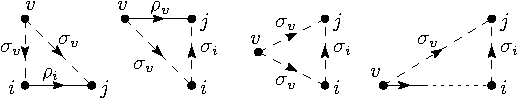
\includegraphics[width=0.9\textwidth]{figures/lower-bound-lemma.pdf}
  \caption{Sketch of the four cases distinguished in the proof of
    Lemma~\ref{lb_lemma}. Arc weights are given and disjunctive arcs
    $\mathcal{O}(\pi)$ are drawn with a dashed line.}\label{fig:lb_lemma}
\end{figure}


\begin{proposition}\label{prop:exhaustive}
  Consider an instance of~\eqref{eq:single_intersection_scheduling} with $\rho_{i} = \rho$ and $\sigma_{i} = \sigma > \rho$ for all
  $i \in \mathcal{N}$. Suppose $y$ is an optimal schedule with
  $y_{i^{*}} + \rho \geq r_{j^{*}}$, for some $(i^{*},j^{*}) \in \mathcal{C}$, then
  $j^{*}$ follows immediately after $i^{*}$, so $y_{i^{*}} + \rho = y_{j^{*}}$.
\end{proposition}
\begin{proof}
  Suppose the ordering $\pi$ of $y$ is such that
  $\pi^{-1}(i^{*}) + 1 < \pi^{-1}(j^{*})$.
  %
  Let $\mathcal{I}(i,j) = \{ i, \pi(\pi^{-1}(i) + 1), \dots, j \}$ be the set of
  vehicles between $i$ and $j$.
  %
  Let $f = \pi(1)$ and $e = \pi(|\mathcal{N}|)$ be the first and last vehicles,
  respectively, and set $u = \pi^{-1}(i^{*}) + 1$ and $v = \pi^{-1}(j^{*}) - 1$, see also Figure~\ref{fig:platoon-preservation-diagram}.
  Construct new ordering $\pi'$ by moving vehicle $j^{*}$ forward
  by $|\mathcal{I}(u,v)|$ places and let $y'$ denote the corresponding schedule.
  %
  We have $y_{i} = y'_{i}$ for all $i \in \mathcal{I}(f, i^{*})$, so these do not
  contribute to any difference in the objective.
  %
  Using Proposition~\ref{prop:active-schedule} and Lemma~\ref{lb_lemma}, we compute
  \begin{align*}
    y'_{j^{*}} &= \max \{ r_{j^{*}}, y_{i^{*}} + \rho \} = y_{i^{*}} + \rho , \\
    y_{u} &= \max \{ r_{u}, y_{i^{*}} + \sigma \} , \\
    y'_{u} &= \max \{ r_{u}, y_{i^{*}} + \rho + \sigma \} ,
  \end{align*}
  where we used that $y_{i^{*}} + \rho \geq r_{j^{*}}$ by assumption.
  %
  Note that we have
  $y_{i^{*}} + \sigma + (|\mathcal{I}(u,v)| - 1) \rho \leq y_{v}$, regardless of the
  type of arcs between consecutive vehicles in $\mathcal{I}(u,v)$. Therefore,
  \begin{align*}
    y_{j^{*}} - y'_{j^{*}} \geq y_{v} + \sigma - y_{i^{*}} - \rho \geq 2 \sigma + (|\mathcal{I}(u,v)| - 2) \rho .
  \end{align*}

  We now show that $y'_{k} \geq y_{k}$ and $y'_{k} - y'_{j^{*}} \leq y_{k} - y_{i^{*}}$ for every $k \in \mathcal{I}(u,v)$.
  For $k = u$, it is clear that $y'_{u} \geq y_{u}$ and
  \begin{align*}
    y'_{u} - y'_{j^{*}} = \max \{ r_{u} - (y_{i^{*}} + \rho), \sigma \} \leq \max \{ r_{u} - y_{i^{*}}, \sigma \} = y_{u} - y_{i^{*}}.
  \end{align*}
  Now proceed by induction and let $x$ be the immediate predecessor of $k$ for
  which the inequalities hold, then
  \begin{align*}
    y'_{k} = \max \{ r_{k}, y'_{x} + w(x,k) \} \geq \max \{ r_{k}, y_{x} + w(x,k) \} = y_{k}
  \end{align*}
  and the second inequality follows from
  %\begin{align*}
  %  y'_{k} - y'_{x} = \max \{ r_{k} - y'_{x}, w(x,k) \} &\leq \max \{ r_{k} - y_{x}, w(x,k)\} = y_{k} - y_{x}
  %\end{align*}
  %implies that
  %\begin{align*}
  %  y'_{k} - y'_{j^{*}} = (y'_{k} - y'_{x}) + (y'_{x} - y'_{j^{*}}) \leq (y_{k} - y_{x}) + (y_{x} - y_{i^{*}}) = y_{k} - y_{i^{*}} .
  %\end{align*}
  %
  \begin{align*}
    (y'_{k} - y'_{x}) + (y'_{x} - y'_{j^{*}}) &= \max \{ r_{k} - y'_{x}, w(x,k) \} + (y'_{x} - y'_{j^{*}}) \\
                                             &\leq \max \{ r_{k} - y_{x}, w(x,k) \} + (y_{x} - y_{i^{*}}) \\
                                             &= (y_{k} - y_{x}) + (y_{x} - y_{i^{*}}) .
  \end{align*}

  Let $l$ denote the immediate successor of $j^{*}$, if there is one. Regardless of
  whether $j^{*}$ and $l$ are in the same lane, we have
  $y_{j^{*}} + \rho \leq y_{l}$. We derive
  \begin{align*}
    y'_{v} = y'_{v} - y'_{j^{*}} + y'_{j^{*}} \leq y_{v} - y_{i^{*}} + y'_{j^{*}} = y_{v} + \rho \leq y_{j^{*}} - \sigma + \rho ,
  \end{align*}
  from which follows that $y'_{v} + \sigma \leq y_{l}$,
  %\begin{align*}
  %  y'_{v} + \sigma = (y'_{v} - y'_{j^{*}}) + y'_{j^{*}} + \sigma \leq y_{v} - y_{i^{*}} + y'_{j^{*}} + \sigma = y_{v} + \rho + \sigma \leq y_{j^{*}} + \rho \leq y_{l} ,
  %\end{align*}
  which means that $y_{i} \geq y'_{i}$ for $i \in \mathcal{I}(l, e)$.

  We can now compare the objectives by putting everything together
  \begin{align*}
    \sum_{i \in \mathcal{N}} y_{i} - y'_{i} &=  y_{j^{*}} - y'_{j^{*}} + \sum_{i \in \mathcal{I}(u, v)} y_{i} - y'_{i} + \sum_{i \in \mathcal{I}(l, e)} y_{i} - y'_{i} \\
    &\geq 2 \sigma + (|\mathcal{I}(u,v)| - 2) \rho + \sum_{k \in \mathcal{I}(u,v)} (y_{k} - y_{i^{*}}) - (y'_{k} - y'_{j^{*}}) \\ & \hspace{12em} - |\mathcal{I}(u,v)| (y'_{j^{*}} - y_{i^{*}}) \\
    &\geq 2 \sigma - 2 \rho > 0
  \end{align*}
  which contradicts the assumption that $y$ and $\pi$ were optimal.
  %
  Finally, from Proposition~\ref{prop:active-schedule} and Lemma~\ref{lb_lemma}
  follows that $y_{i^{*}} + \rho = y_{j^{*}}$.
\end{proof}

\begin{figure}[H]
  \centering
  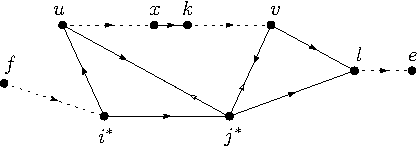
\includegraphics[width=0.8\textwidth]{figures/platoon-preservation-proof-diagram.pdf}
  \caption{Sketch of the nodes and most important arcs used in the proof of
    Proposition~\ref{prop:exhaustive}. Dashed arcs represent chains of
    unspecified length. The two open arrows indicate the new direction of their
    arc under ordering $\pi'$.}\label{fig:platoon-preservation-diagram}
\end{figure}


\subsection*{Branch-and-bound approach}

Optimization problem~\ref{eq:single_intersection_scheduling} can be turned into
a Mixed-Integer Linear Program (MILP) by rewriting the disjunctive constraints using
the well-known big-M method.
%
We introduce a binary decision variable $\gamma_{ij}$ for every
disjunctive pair $\{i, j\} \in \mathcal{D}$.
%
To avoid redundant variables, we first impose some arbitrary ordering of the
disjunctive pairs by defining
\begin{align*}
  \bar{\mathcal{D}} = \{ (i,j) : \{i,j\} \in \mathcal{D}, \; l(i) < l(j) \} ,
\end{align*}
such that for every $(i,j) \in \bar{\mathcal{D}}$, setting $\gamma_{ij} = 0$
corresponds with choosing disjunctive arc $i \rightarrow j$ and
$\gamma_{ij} = 1$ corresponds to $j \rightarrow i$. This yields the following
MILP formulation
%
\begin{align*}
  \min_{y} \quad & \sum_{i \in \mathcal{N}} y_{i} & \\
  \text{s.t.} \quad & r_{i} \leq y_{i} & \text{ for all } i \in \mathcal{N} , \\
  & y_{i} + \rho_{i} \leq y_{j} & \text{ for all } (i,j) \in \mathcal{C} , \label{eq:conjunctions} \\
  & y_{i} + \sigma_{i} \leq y_{j} + \gamma_{ij}M & \text{ for all } (i,j) \in \bar{\mathcal{D}} , \\
  & y_{j} + \sigma_{j} \leq y_{i} + (1 - \gamma_{ij})M & \text{ for all } (i,j) \in \bar{\mathcal{D}} , \\
  & \gamma_{ij} \in \{0, 1\} & \text{ for all } (i,j) \in \bar{\mathcal{D}} ,
\end{align*}
where $M > 0$ is some sufficiently large number, which may depend on the
specific problem instance.

\subsubsection*{Cutting planes}

Consider some disjunctive arc $(i,j) \in \bar{\mathcal{D}}$. Let $i^{<}$ denote
the set of indices on lane $l(i)$ from which is a conjunctive path to $i$.
Similarly, let $j^{>}$ denote the set of indices on lane $l(j)$ to which is a
conjunctive path from $j$.
%
Now suppose $\gamma_{ij} = 0$, so the direction of the arc is $i \rightarrow j$,
then we must clearly also have
\begin{align*}
  p \rightarrow q \equiv \gamma_{pq} = 0 \; \text{ for all } p \in i^{<}, q \in j^{>} .
\end{align*}
Written in terms of the disjunctive variables, this gives us the cutting planes
\begin{align*}
  \sum_{p \in i^{<}, q \in j^{>}} \gamma_{pq} \leq \gamma_{ij} M .
\end{align*}
We refer to these as the \textit{disjunctive cutting planes} and any feasible solution
must satisfy these. {\color{blue} We did not include this type of cutting
  plane in the running time analysis because it is not yet implemented.}

Next, we consider two types of cutting planes that follow from the necessary condition
for optimality in Propositon~\ref{prop:exhaustive}.
%
Suppose $y$ is an optimal schedule. If we have $y_{i} + \rho \geq r_{j}$ for
some conjunctive pair $(i,j) \in \mathcal{C}$, we must have $y_{i} + \rho = y_{j}$
by Proposition~\ref{prop:exhaustive}. In order to model this rule, we first introduce a binary
variable $\beta_{ij}$ that satisfies
\begin{align*}
  \beta_{ij} = 0 &\iff y_{i} + \rho < r_{j} , \\
  \beta_{ij} = 1 &\iff y_{i} + \rho \geq r_{j} ,
\end{align*}
which can be enforced by adding the constraints
\begin{align*}
  y_{i} + \rho &< r_{j} + \beta_{ij}M , \\
  y_{i} + \rho &\geq r_{j} - (1 - \beta_{ij}) M .
\end{align*}
Now observe that the rule is enforced by adding the following cutting plane
\begin{align*}
  y_{i} + \rho &\geq y_{j} - (1 - \beta_{ij}) M .
\end{align*}
We refer to the above cutting planes as \textit{type I}.
%
We can add more cutting planes on the disjunctive decision variables, because
whenever $\beta_{ij} = 1$, the directions of the disjunctive arcs $i \rightarrow k$ and
$j \rightarrow k$ must be the same for every other vertex $k \in \mathcal{N}$. Therefore,
consider the following constraints
\begin{align*}
  \beta_{ij} + (1 - \gamma_{ik}) + \gamma_{jk} \leq 2 , \\
  \beta_{ij} + \gamma_{ik} + (1 - \gamma_{jk}) \leq 2 ,
\end{align*}
for every $(i,j) \in \mathcal{C}$ and for every $k \in \mathcal{N}$ with $l(k) \neq l(i) = l(j)$.
These are the \textit{type II} cutting planes.

%\vspace{0.5em} \noindent \textbf{Preprocessing.}
%We now show how Proposition~\ref{prop:exhaustive} can also be used as a preprocessing step.
%Vehicles are ``glued'' together, but then the contribution of this platoon to
%the objective also needs to be scaled accordingly.

\subsubsection*{Running time analysis}

First, we define some classes of problem instances that we will use as a benchmark.
%
Instances are generated by sampling $g_{i}$ and $\rho_{i}$ and setting
\begin{align*}
  r_{i} = \sum_{k=1}^{k(i)} g_{i} + \sum_{k=1}^{k(i) - 1} \rho_{i} ,
\end{align*}
for each $i \in \mathcal{N}$.
%
The parameters are as given in Table~\ref{tab:params}. For each set of instances, we report
solving times in Table~\ref{tab:running_times}. It is clear that adding cutting planes for the
larger instances is beneficial. However, it seems that it is not always worth
adding cutting planes of type II.


\subsubsection*{Alternatives}
The number of disjunctive variables in the MILP formulation is of order $O(|\mathcal{N}|^{2})$.
%
The existence of the disjunctive cutting planes shows that there is a lot of redundancy in this formulation: roughly speaking, the decision to choose disjunctive arc $i \rightarrow j$ involves setting $O(\mathcal{N})$ other disjunctive decision variables.
%
Therefore, it might be possible to find more compact equivalent formulations.
%
Alternatively, instead of relying on a MILP formulation and the capabilities of
modern MILP solvers, a tailored branch-and-bround algorithm can be considered.



\subsection*{Constructive heuristics}

% constructive scheduling
Methods that rely on branch-and-bound techniques guarantee to find an optimal
solution, but their running time scale very badly with increasing instance
sizes. Therefore, we are interested in developing heuristics to obtain good
approximations in reasonable time. A common approach for developing such
heuristics in the scheduling literature is to incrementally construct a schedule
by fixing one job starting time at each step, so we will consider incrementally
constructing a vehicle ordering.

To this end, we define partial ordering $\pi$ to be a \textit{partial permutation} of
$\mathcal{N}$, which is a sequence of elements from some subset
$\mathcal{N}(\pi) \subset \mathcal{N}$.
%
Let $\pi$ be a partial ordering of length $n$ and let
$i \notin \mathcal{N}(\pi)$, then we use $\pi' = \pi \mdoubleplus i$ to denote
the concatenation of sequence $\pi$ with $i$, so $\pi'_{1:n} = \pi_{1:n}$ and
$\pi'_{n+1} = i$. Furthermore, recursively define the concatenation of two
sequences by
$\pi \mdoubleplus \pi' = ( \pi \mdoubleplus \pi'_{1} ) \mdoubleplus \pi'_{2:m}$,
where $m$ is the length of $\pi'$.

For each partial ordering $\pi$, the corresponding disjunctive graph $G(\pi)$ is
incomplete, meaning that some of the disjunctive arcs have not yet been added.
Nevertheless, observe that $\text{LB}_{\pi}(i)$ is still defined for every
$i \in \mathcal{N}$.
%
Let $\text{obj}(\pi)$ denote the objective of a complete ordering $\pi$, then
the following rule for constructing partial orderings follows from
Proposition~\ref{prop:exhaustive}.

\begin{corollary}\label{prop:exhaustive_partial}
  % same assumptions as in prop:exhaustive
  Consider an instance of~\eqref{eq:single_intersection_scheduling} with
  $\rho_{i} = \rho$ and $\sigma_{i} = \sigma > \rho$ for all
  $i \in \mathcal{N}$.
  %
  Let $\pi$ be a partial ordering of length $n$ with optimal completion schedule
  \begin{align*}
    \pi^{*} = \arg\min_{\pi'} \;  \mathrm{obj}(\pi \mdoubleplus \pi') .
  \end{align*}
  %
  If $(\pi(n),j) \in \mathcal{C}$ exists and satisfies
  $\text{LB}_{{\pi}}(\pi(n)) + \rho_{\pi(n)} \geq r_{j}$, then $\pi^{*}(1) = j$.
\end{corollary}

% lane ordering automaton
Observe that ordering vehicles is equivalent to ordering the lanes, due to the
conjunctive constraints. We will define heuristics in terms of repeatedly
choosing the next lane. It may be helpful to model this as a deterministic
finite-state automaton, where the set of lane indices acts as the input alphabet
$\Sigma = \{ 1, \dots, n \}$, where $n$ denotes the number of lanes. Let $S$
denote the state space and let $\delta: S \times \Sigma \rightarrow S$ denote
the state-transition function.

% states
Let $s$ denote an instance of~\eqref{eq:single_intersection_scheduling}. We
consider $s$ to be a fixed part of the state, so it does not change with state
transitions.
The other part of the state is the current partial ordering $\pi$.
% transitions
The transitions of the automaton are very simple. Let $(s, \pi) \in S$ denote
the current state and let $l \in \Sigma$ denote the next symbol. Let
$i \in \mathcal{N} \setminus \mathcal{N}(\pi)$ denote the next unscheduled vehicle on lane $l$,
then the system transitions to $(s, \pi \mdoubleplus i)$. If no such vehicle exists, the
transition is undefined.
%
% multi-step transition
% With a little abuse of notation, let $\delta(s, \eta) = \delta(s_{0}, \eta)$ denote the
% state that we obtain after applying sequence $\eta$ to the automaton with initial
% state $s_{0} = (s, \varnothing)$, which generalizes the single step transition function by
% recursively defining
% \begin{align*}
%   \delta(s_{0}, \eta_{1:t}) = \delta(\delta(s_{0}, \eta_{1:t-1}), \eta_{t}) .
% \end{align*}
%
Therefore, an input sequence $\eta$ of lanes is called a \textit{valid lane
  order} whenever it is of length
\begin{align*}
  N = \sum_{l \in \Sigma} n_{l}
\end{align*}
and contains precisely $n_l = |\{ i \in \mathcal{N} : l(i) = l \}|$ occurrences
of lane $l \in \Sigma$. Given problem instance $s$, let $y_{\eta}(s)$ denote the
schedule corresponding to lane order $\eta$. We say that lane order $\eta$ is
optimal whenever $y_{\eta}(s)$ is optimal. Observe that an optimal lane order
must exist for every instance $s$, since we can simply derive the lane order
from an optimal vehicle order.

Instead of mapping an instance $s$ directly to some optimal lane order, we
consider a mapping $p : S \rightarrow \Sigma$ such that setting
$s_{0} = (s, \varnothing)$ and repeatedly evaluating
\begin{align*}
  s_{t} = \delta(s_{t-1}, p(s_{t-1}))
\end{align*}
yields a final state $s_{N}(s, \pi^{*})$ with optimal schedule $\pi^{*}$.
Observe that this mapping must exist, because given some optimal lane order
$\eta^{*}$, we can set $p(s_{t}) = \eta^{*}_{t+1}$, for every $t \in \{0, \dots, N-1\}$.

We do not hope to find an explicit representation of $p$, but our aim is to find
good heuristic approximations.
For example, consider the following simple \textit{threshold rule}.
%
Let $\pi$ denote a partial schedule of length $n$, so $i=\pi(n)$ is the last
scheduled vehicle on some lane $l=l(i)$, then define
\begin{align*}
  p_{\tau}(s, \pi) = \begin{cases}
                l \quad &\text{ if } \text{LB}_{\pi}(i) + \rho_{i} + \tau \geq r_{j} \text{ and } (i,j) \in \mathcal{C} , \\
                \texttt{next}(\pi) & \text{ otherwise, }
              \end{cases}
\end{align*}
for some threshold $\tau \geq 0$. The expression $\texttt{next}(\pi)$ represents some lane
other than $l$ with unscheduled vehicles left.
%
This heuristic satisfies the rule of
Corollary~\ref{prop:exhaustive_partial} for any $\tau$ and may as such be
interpreted as a relaxation of this rule.


\subsection*{Behavioral cloning}

% We model the conditional distribution
% $p_{\theta}(\eta | s)$ of the optimal lane sequence given a problem instance $s$
% and we factorize it as
% %
% \begin{align*}
%   p_{\theta} (\eta \, | \, s) = \prod_{t=1}^{N} p_{\theta}(\eta_{t} \, | \; \delta(s, \eta_{1:t-1})) ,
% \end{align*}
% %
% where $\theta$ denotes the model parameters.

Instead of explicitly formulating heuristics using elementary rules, we will now
consider a data-driven approach. To this end, we model the conditional
distribution $p_{\theta}(\eta_{t+1} | s_{t})$ with model parameters $\theta$.
%
Consider an instance $s$ and some optimal lane sequence $\eta$ with
corresponding states defined as $s_{t+1} = \delta(s_{t}, \eta_{t+1})$ for
$t \in \{0, \dots, N-1\}$. The resulting set of pairs $(s_{t}, \eta_{t+1})$ can be
used to learn $p_{\theta}$ in a supervised fashion by treating it as a classification
task.

% inference
Schedules are generated by employing \textit{greedy inference} as follows. The
model $p_{\theta}$ provides a distribution over lanes. We ignore lanes that have
no unscheduled vehicles left and take the argmax of the remaining probabilities.
We will denote the corresponding complete schedule by $\hat{y}_{\theta}(s)$.

Next, we discuss two ways of parameterizing the model. In both cases, we first
derive, for every $l \in \Sigma$, a \textit{lane embedding} $h(s_{t}, l)$ based on the current
non-final state $s_{t} = (s, \pi_{t})$ of the automaton. These are then arranged
into a \textit{state embedding} $h(s_{t})$ as follows. Let $\eta_{t}$ be the lane that was
chosen last, then we apply the following \textit{lane cycling} trick in order to keep the
most recent lane in the same position of the state embedding, by defining
\begin{align*}
  h_{l}(s_{t}) = h(s_{t}, \; l - \eta_{t} \; \mathrm{mod} \; |\Sigma|) ,
\end{align*}
for every $l \in \Sigma$.
%
This state embedding is then mapped to a probability distribution
\begin{align*}
  p_{\theta}(\eta_{t+1} | s_{t}) = f_{\theta}(h(s_{t})) ,
\end{align*}
where $f_{\theta}$ is a fully connected neural network.


\subsubsection*{Padded embedding}
%
Let $k_{\pi}(l)$ denote the first unscheduled vehicle in lane $l$ under the partial schedule $\pi_{t}$.
Denote the smallest lower bound of unscheduled vehicles as
\begin{align*}
  T_{\pi} = \min_{i \in \mathcal{N} \setminus \mathcal{N}(\pi)} \text{LB}_{\pi}(i) .
\end{align*}
Let the \textit{horizon} of lane $l$ be defined as
\begin{align*}
  h'(s_{t}, l) = ( \text{LB}_{\pi_{t}}(k_{\pi_{t}}(l)) - T_{\pi_{t}}, \dots, \text{LB}_{\pi_{t}}(n_{l}) - T_{\pi_{t}} ) .
\end{align*}
%
Observe that horizons can be of arbitrary dimension. Therefore, we restrict each
horizon to a fixed length $\Gamma$ and use zero padding. More precisely, given a
sequence $x = (x_{1}, \dots, x_{n})$ of length $n$, define the padding
operator
\begin{align*}
  \text{pad}(x, \Gamma) = \begin{cases}
                            (x_{1}, \dots, x_{\Gamma}) &\text{ if } \Gamma \leq n,  \\
                            (x_{1}, \dots, x_{n}) \mdoubleplus (\Gamma - n) * (0) &\text{ otherwise, }
                            \end{cases}
\end{align*}
where we use the notation $n * (0)$ to mean a sequence of $n$ zeros.
%
The lane embedding is then given by
\begin{align*}
  h(s_{t}, l) = \text{pad}(h'(s_{t}, l), \Gamma).
\end{align*}
%

\subsubsection*{Recurrent embedding}

To avoid the zero padding operation, which can be problematic for states that
are almost done, we can employ a recurrent architecture that is agnostic to the
number of remaining unscheduled vehicles. Each variable-length horizon
$h'(s_{t}, l)$ is simply transformed into the fixed-length vector by an Elman
RNN by taking the output at the last step. {\color{blue} Need to further specify
  this, but the current implementation is working.}
% \begin{align*}
%   h(s_{t}, l) = \text{RNN}(h'(s_{t}, l)) .
% \end{align*}


\subsection*{Experiments}

We consider an intersection with two approaching lanes. For each test instance
set from Table~\ref{tab:params}, we sample 1000 instances from the same
distribution. We solve each instance to optimality using a branch-and-bound
method to obtain the training data set $\mathcal{X}$, consisting of all the
pairs $(s_{t}, \eta_{t+1})$ of state and next lane belonging to the optimal
schedules.

% threshold heuristic fitting
We fit the simple threshold heuristic to $\mathcal{X}$ by finding the value of
$\tau$ with the lowest mean objective using a simple grid search. The fitted values
are given in Table~\ref{tab:tau_opt}. Note that these values are all remarkably
close, so we wonder if there is any dependency on $\rho_{i}$ or $\sigma$,
because these are the only variables kept constant among the instance sets.


% neural heuristics fitting
In order to fit the model parameters of the neural models, we interpret
$p_{\theta}(s_{t})$ as the probability of choosing the first lane and use the
binary cross entropy loss, defined as
\begin{align*}
  - \frac{1}{|\mathcal{X}|} \sum_{(s_{t}, \eta_{t+1}) \in \mathcal{X}} \mathds{1}\{\eta_{t+1} = 1\} \log(p_{\theta}(s_{t})) + \mathds{1}\{\eta_{t+1} = 2\} \log(1 - p_{\theta}(s_{t})) ,
\end{align*}
where $\mathds{1}(\cdot)$ denotes the indicator function.
%
We use 5 epochs with batch size 10 and we use learning rate $10^{-3}$ with the
Adam optimizer.

% evaluation
Let $\mathcal{Y}$ denote one of the test instances set. Let $\text{obj}(y)$
denote the objective of schedule $y$, and let $\hat{y}$ denote the schedule
obtained from a heuristic, then Table~\ref{tab:objectives} reports on the
average approximation ratio defined as
\begin{align*}
  \alpha_{\text{approx}} = \frac{1}{|\mathcal{Y}|} \sum_{s \in \mathcal{Y}} \text{obj}(\hat{y}(s)) \; / \; \text{obj}(y^{*}(s))
\end{align*}
and the fraction of instances that are solved to optimality, which
we define as
\begin{align*}
  \alpha_{\text{opt}} = \frac{1}{|\mathcal{Y}|} \sum_{s \in \mathcal{Y}} \mathds{1}\{ \text{obj}(\hat{y}(s)) = \text{obj}(y^{*}(s)) \} .
\end{align*}




{\color{blue}
\subsection*{Further analysis}

\begin{itemize}
  \item We are particularly interested in the ability of the model to generalize
        to instances with more vehicles, because this is where the MILP solving
        time begins to become prohibitive.

  \item The rule of Corollary~\ref{prop:exhaustive_partial} is currently not
        used in the evaluation of the heuristics.

  \item It might be insightful to compare the model probability of the computed
        greedy schedule to the model probability of the optimal solution
        computed using mixed-integer linear programming. This provides us an
        indication of model fit and whether greedy inference is good enough or
        methods like beam search might be necessary.

  \item It might be interesting to analyze the feature attribution of the neural
        network using a method like Integrated Gradients.
\end{itemize}
}

\newpage

\begin{table}[H]
  \caption{Specification of test instance sets. The total number of vehicles is
    shown as the sum of the number of vehicles per lane $\sum n_{l}$. Every
    instance has switch-over time $\sigma = 2$. {\color{blue} I plan on including
      some more (multi-modal) distributions, but I am still thinking about a
      suitable presentation; varying the instance size $|\mathcal{N}|$ is
      interesting for the analysis of branch-and-bound, but varying the
      distributions is mainly interesting for the heuristics.}}
    \label{tab:params}
    % Change switch-over time to $s=1$ ``without loss of generality''.
    % To give an idea of the distribution, the first few arrivals (truncation at
    % $40$) of the first lane are shown for some sample instance.

  \centering
  \begin{tabular}[t]{c c c c c c}
    \toprule
    set id & size & $|\mathcal{N}|$ & $g_{i}$ & $\rho_{i}$ \\
    \midrule

    1 & 100 & $10 + 10$ & $\text{Uni}(0, 4)$ & $1$ \\
    2 & 100 & $15 + 15$ & $\text{Uni}(0, 4)$ & $1$ \\
    3 & 100 & $20 + 20$ & $\text{Uni}(0, 4)$ & $1$ \\
    4 & 100 & $25 + 25$ & $\text{Uni}(0, 4)$ & $1$ \\ % too big for free Gurobi version

    5 & 100 & $10 + 10$ & $\text{Exp}(2)$    & $1$ \\
    6 & 100 & $15 + 15$ & $\text{Exp}(2)$    & $1$ \\

    \bottomrule
  \end{tabular}
\end{table}

% uses knitr to generate nice tables
% silent package loading


\begin{knitrout}
\definecolor{shadecolor}{rgb}{0.969, 0.969, 0.969}\color{fgcolor}\begin{table}

\caption{\label{tab:unnamed-chunk-2}Solving times of Gurobi on the different sets of instances. Mean and standard deviation are given for the MILP without cutting planes (``plain''), type I cutting planes or both types of cutting planes. \label{tab:running_times}}
\centering
\begin{tabular}[t]{rlll}
\toprule
set id & plain & type I & type I + II\\
\midrule
1 & 0.084 $\pm$ 0.011 & 0.078 $\pm$ 0.004 & 0.087 $\pm$ 0.022\\
2 & 0.452 $\pm$ 0.007 & 0.314 $\pm$ 0.028 & 0.299 $\pm$ 0.134\\
3 & 2.525 $\pm$ 0.073 & 0.764 $\pm$ 0.267 & 0.837 $\pm$ 0.109\\
4 & 8.688 $\pm$ 5.326 & 2.486 $\pm$ 0.892 & 1.585 $\pm$ 0.045\\
\bottomrule
\end{tabular}
\end{table}

\end{knitrout}

% silent package loading


\begin{knitrout}
\definecolor{shadecolor}{rgb}{0.969, 0.969, 0.969}\color{fgcolor}\begin{table}

\caption{\label{tab:unnamed-chunk-2}Approximation ratio for the heuristics. \label{tab:objectives}}
\centering
\begin{tabular}[t]{rr}
\toprule
set id & threshold $\tau = 1.2$\\
\midrule
1 & 1.026537\\
2 & 1.017220\\
3 & 1.011988\\
4 & 1.011209\\
6 & 1.026830\\
\addlinespace
7 & 1.026359\\
\bottomrule
\end{tabular}
\end{table}

\end{knitrout}

% silent package loading


\begin{knitrout}
\definecolor{shadecolor}{rgb}{0.969, 0.969, 0.969}\color{fgcolor}\begin{table}[H]
\centering
\caption{\label{tab:unnamed-chunk-2}Optimal values of threshold parameter $\tau$ of the threshold
    heuristic, fitted using a simple grid search on each training data
    set.  \label{tab:tau_opt}}
\centering
\begin{tabular}[t]{ccccccc}
\toprule
set id & 1 & 2 & 3 & 4 & 5 & 6\\
\midrule
$\tau$ & 1.10 & 1.10 & 1.00 & 0.90 & 1.10 & 1.10\\
\bottomrule
\end{tabular}
\end{table}

\end{knitrout}


%\newpage
%\subsection*{Reinforcement learning}
%
%If we define rewards for the transitions
%\begin{align*}
%  r : S \times \Sigma \rightarrow \mathbb{R} ,
%\end{align*}
%then we obtain a deterministic Markov Decision Process.


%\section*{Related Literature}
%
%Discuss the paper ``Machine Learning for Combinatorial Optimization: a
%Methodological Tour d'Horizon''~\cite{bengioMachineLearningCombinatorial2020}.
%%
%Learning through behavioral cloning.
%Learning through reinforcement learning, requires the definition of rewards.
%Machine learning for end-to-end algorithm or in parts of branch-and-bound algorithms.

\newpage

\section*{Implementation details}

The code that was used for this report can be found at
\begin{quote}
\url{https://github.com/jeroenvanriel/traffic-scheduling}
\end{quote}
The \texttt{ordering} directory contains the main model definitions and analyses.
A short description of the most important files is given below.

\vspace{1em}
\hrule
\begin{description}
  \item[generate\_instances.py] Generate training and test sets.
  \item[exact.py] Solve instances to optimality using MILP with different settings of cutting planes.
  \item[automaton.py] Definition of the finite-state automaton. Instances of class \texttt{Automaton} are treated as the \textit{state} and contain the state variables
        \begin{description}[leftmargin=!,labelwidth=5em]
          \item[\texttt{N}]  number of lanes,
          \item[\texttt{K}]  number of available vehicles per lane,
          \item[\texttt{k}]  number of scheduled vehicles per lane,
          \item[\texttt{y}]  current schedule $\pi$,
          \item[\texttt{LB}] lower bounds $\pi_{\pi}$ for the current schedule $\pi$,
          \item[\texttt{last\_lane}] last input symbol $l \in \Sigma$.
        \end{description}
  \item[util.py] Contains a set of helper functions, the most important ones being
        \begin{description}[leftmargin=!,labelwidth=7em]
          \item[\texttt{plot\_schedule}]  plot (partial) schedules(s) given some instance,
          \item[\texttt{LB}]  compute $LB_{\pi}(i)$ for every $i \in \mathcal{N}$,
          \item[\texttt{lane\_order}]  given some schedule $y$, compute $\eta$ such that $y_{\eta}(s) = y$.
        \end{description}
  \item[model.py] Definition of the neural network models with padded and recurrent embeddings.
  \item[neural\_heuristic.ipynb] Training and evaluation of the neural heuristics.
  \item[threshold.py] Definition of the threshold rule heuristic.
  \item[threshold\_heuristic.ipynb] Fitting $\tau$ and evaluation of threshold heuristic.
\end{description}
\hrule

\vspace{1em}
Recall that instances of
problem~\eqref{eq:single_intersection_scheduling} are completely characterized
by
\begin{align*}
  s = (\mathcal{N}, \rho, \sigma, r) .
\end{align*}
Throughout the code, it is assumed that
\begin{align*}
  \sigma_{i} = \rho_{i} + s ,
\end{align*}
because this allows us to use the result from Lemma~\ref{lb_lemma}.
Therefore, instances are represented by specifying earliest crossing time
$r_{i}$, length $\rho_{i}$ and \textit{switch-over} time $s$.
We will refer to earliest crossing time as the \textit{release time} of the vehicle.
Both release times and lengths are specified as nested lists, where each inner list corresponds to a lane.
Instances are represented in the code as basic dictionaries of the form
\begin{figure}[H]
\centering
\begin{cminted}
instance = {
    'release': [[1, 2, 4], [1, 2]],
    'length':  [[1, 2, 1], [1, 1]],
    'switch':  2
}
\end{cminted}
\end{figure}

The automaton keeps track of $\text{LB}_{\pi}(i)$ for each node $i$, given the
current partial ordering. It provides these values as basic observations. We
transform these into the desired observations for training our heuristic.
%
The method \texttt{Automaton.exhaustive(lane)} returns whether the rule of
Proposition~\ref{prop:exhaustive_partial} applies to the given lane.

In \texttt{model.py}, the \texttt{state\_transform} method of each embedding
class encodes the state of the automaton into a PyTorch Tensor. The
\texttt{action\_transform} method takes the output logit of the neural network
to produce a lane index. This is necessary to implement the lane cycling trick.
We also need the inverse of this transform (\texttt{inverse\_action\_transform})
to translate optimal next lane indices to actions for supervised learning.

Instances and (partial) schedules can be visualized by \texttt{util.plot\_schedule}.
For example, the instance above together with the optimal solution is shown in
the following figure.
\begin{figure}[H]
\centering
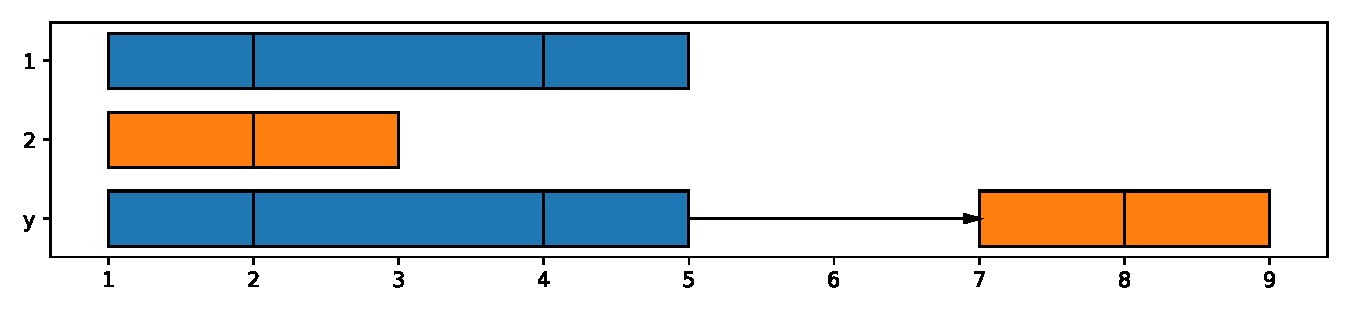
\includegraphics[width=0.9\textwidth]{figures/example_schedule.pdf}
\end{figure}
\noindent
Each vehicle is drawn as a rectangle, whose width represents $\rho_{i}$. The color
of each rectangle corresponds to its lane. The first two rows of the figure
visualize the instance specification and the last row visualizes the optimal
schedule $y$. The arrow visualizes the switch-over time $s$.

\section*{Bibliographical notes}

The disjunctive graph is a common formalism used for job shop scheduling
problems (see Chapter 7 of~\cite{pinedoSchedulingTheoryAlgorithms2016}), to
which our crossing time scheduling problem is related. Furthermore, in
scheduling theory terminology, the result of
Proposition~\ref{prop:active-schedule} says that optimal schedules are
necessarily \textit{semi-active schedules}, see Definition 2.3.5
in~\cite{pinedoSchedulingTheoryAlgorithms2016}.
%
The rule for optimal orderings (Proposition~\ref{prop:exhaustive}) is equivalent
to the \textit{Platoon Preservation Theorem} of
Limpens~\cite{limpensOnlinePlatoonForming2023}.

Machine learning has been used extensively to solve combinatorial problems, see
for example the seminal paper~\cite{belloNeuralCombinatorialOptimization2017} and surveys~\cite{bengioMachineLearningCombinatorial2020,mazyavkinaReinforcementLearningCombinatorial2020}.

\bibliography{references}
\bibliographystyle{ieeetr}


\end{document}

% to enable the minted package
% Local Variables:
% TeX-command-extra-options: "-shell-escape"
% End:
